\subsection{User Interfaces}
DREAM contains two main interfaces: mobile application and webapp interface.
In both interfaces, all three actors can perform the same operations.
However, it should be noted that certain features are more comfortable to use only from a certain interface.
The following mockups will give a more detailed description in terms of interfaces.


\subsubsection{WebApp Registration page}

\begin{figure}[H]
   \centering
  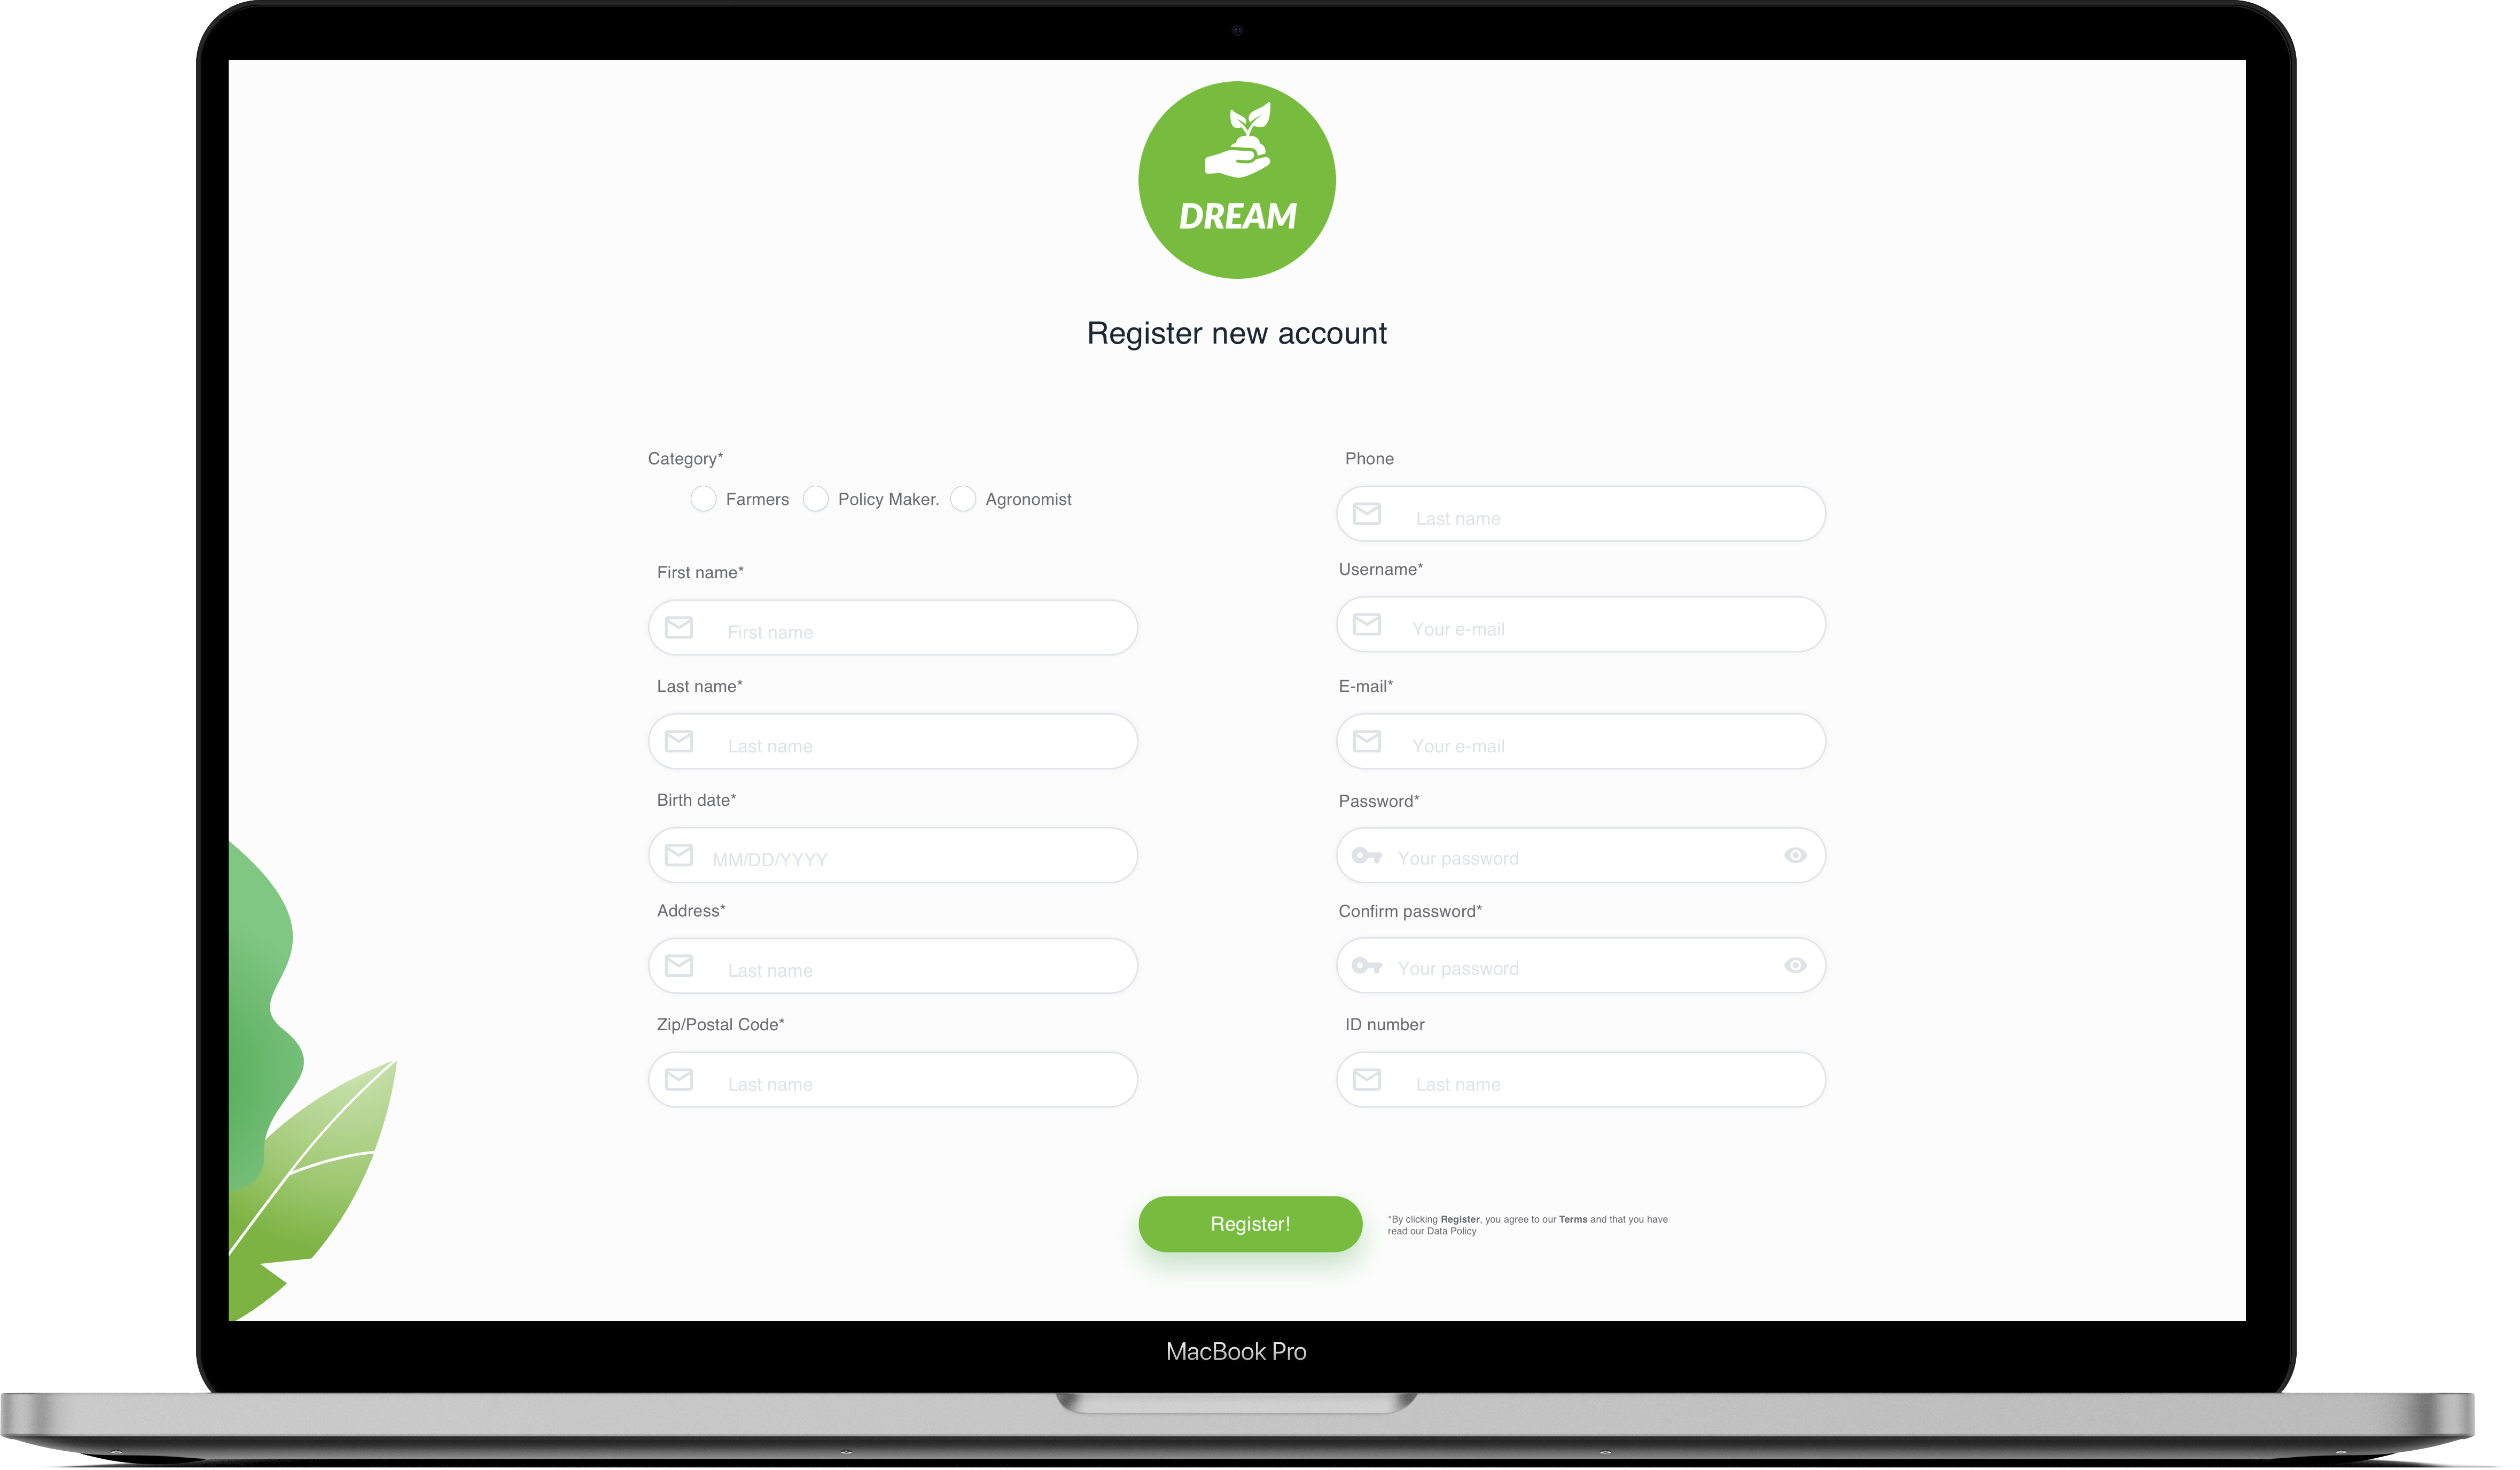
\includegraphics[width=140mm,scale=0.9]{./Images//Mocks/WebApp/Registration.png}
  \caption{WebApp Registration page}
\end{figure}

The three actors can register to DREAM through this registration page, where there are some required fields, and some other fields according to radio button selected corresponding to their role. Registration is completed by accepting term and conditions, and by confirming the following mail.

\subsubsection{WebApp Login page}

\begin{figure}[H]
  \centering
  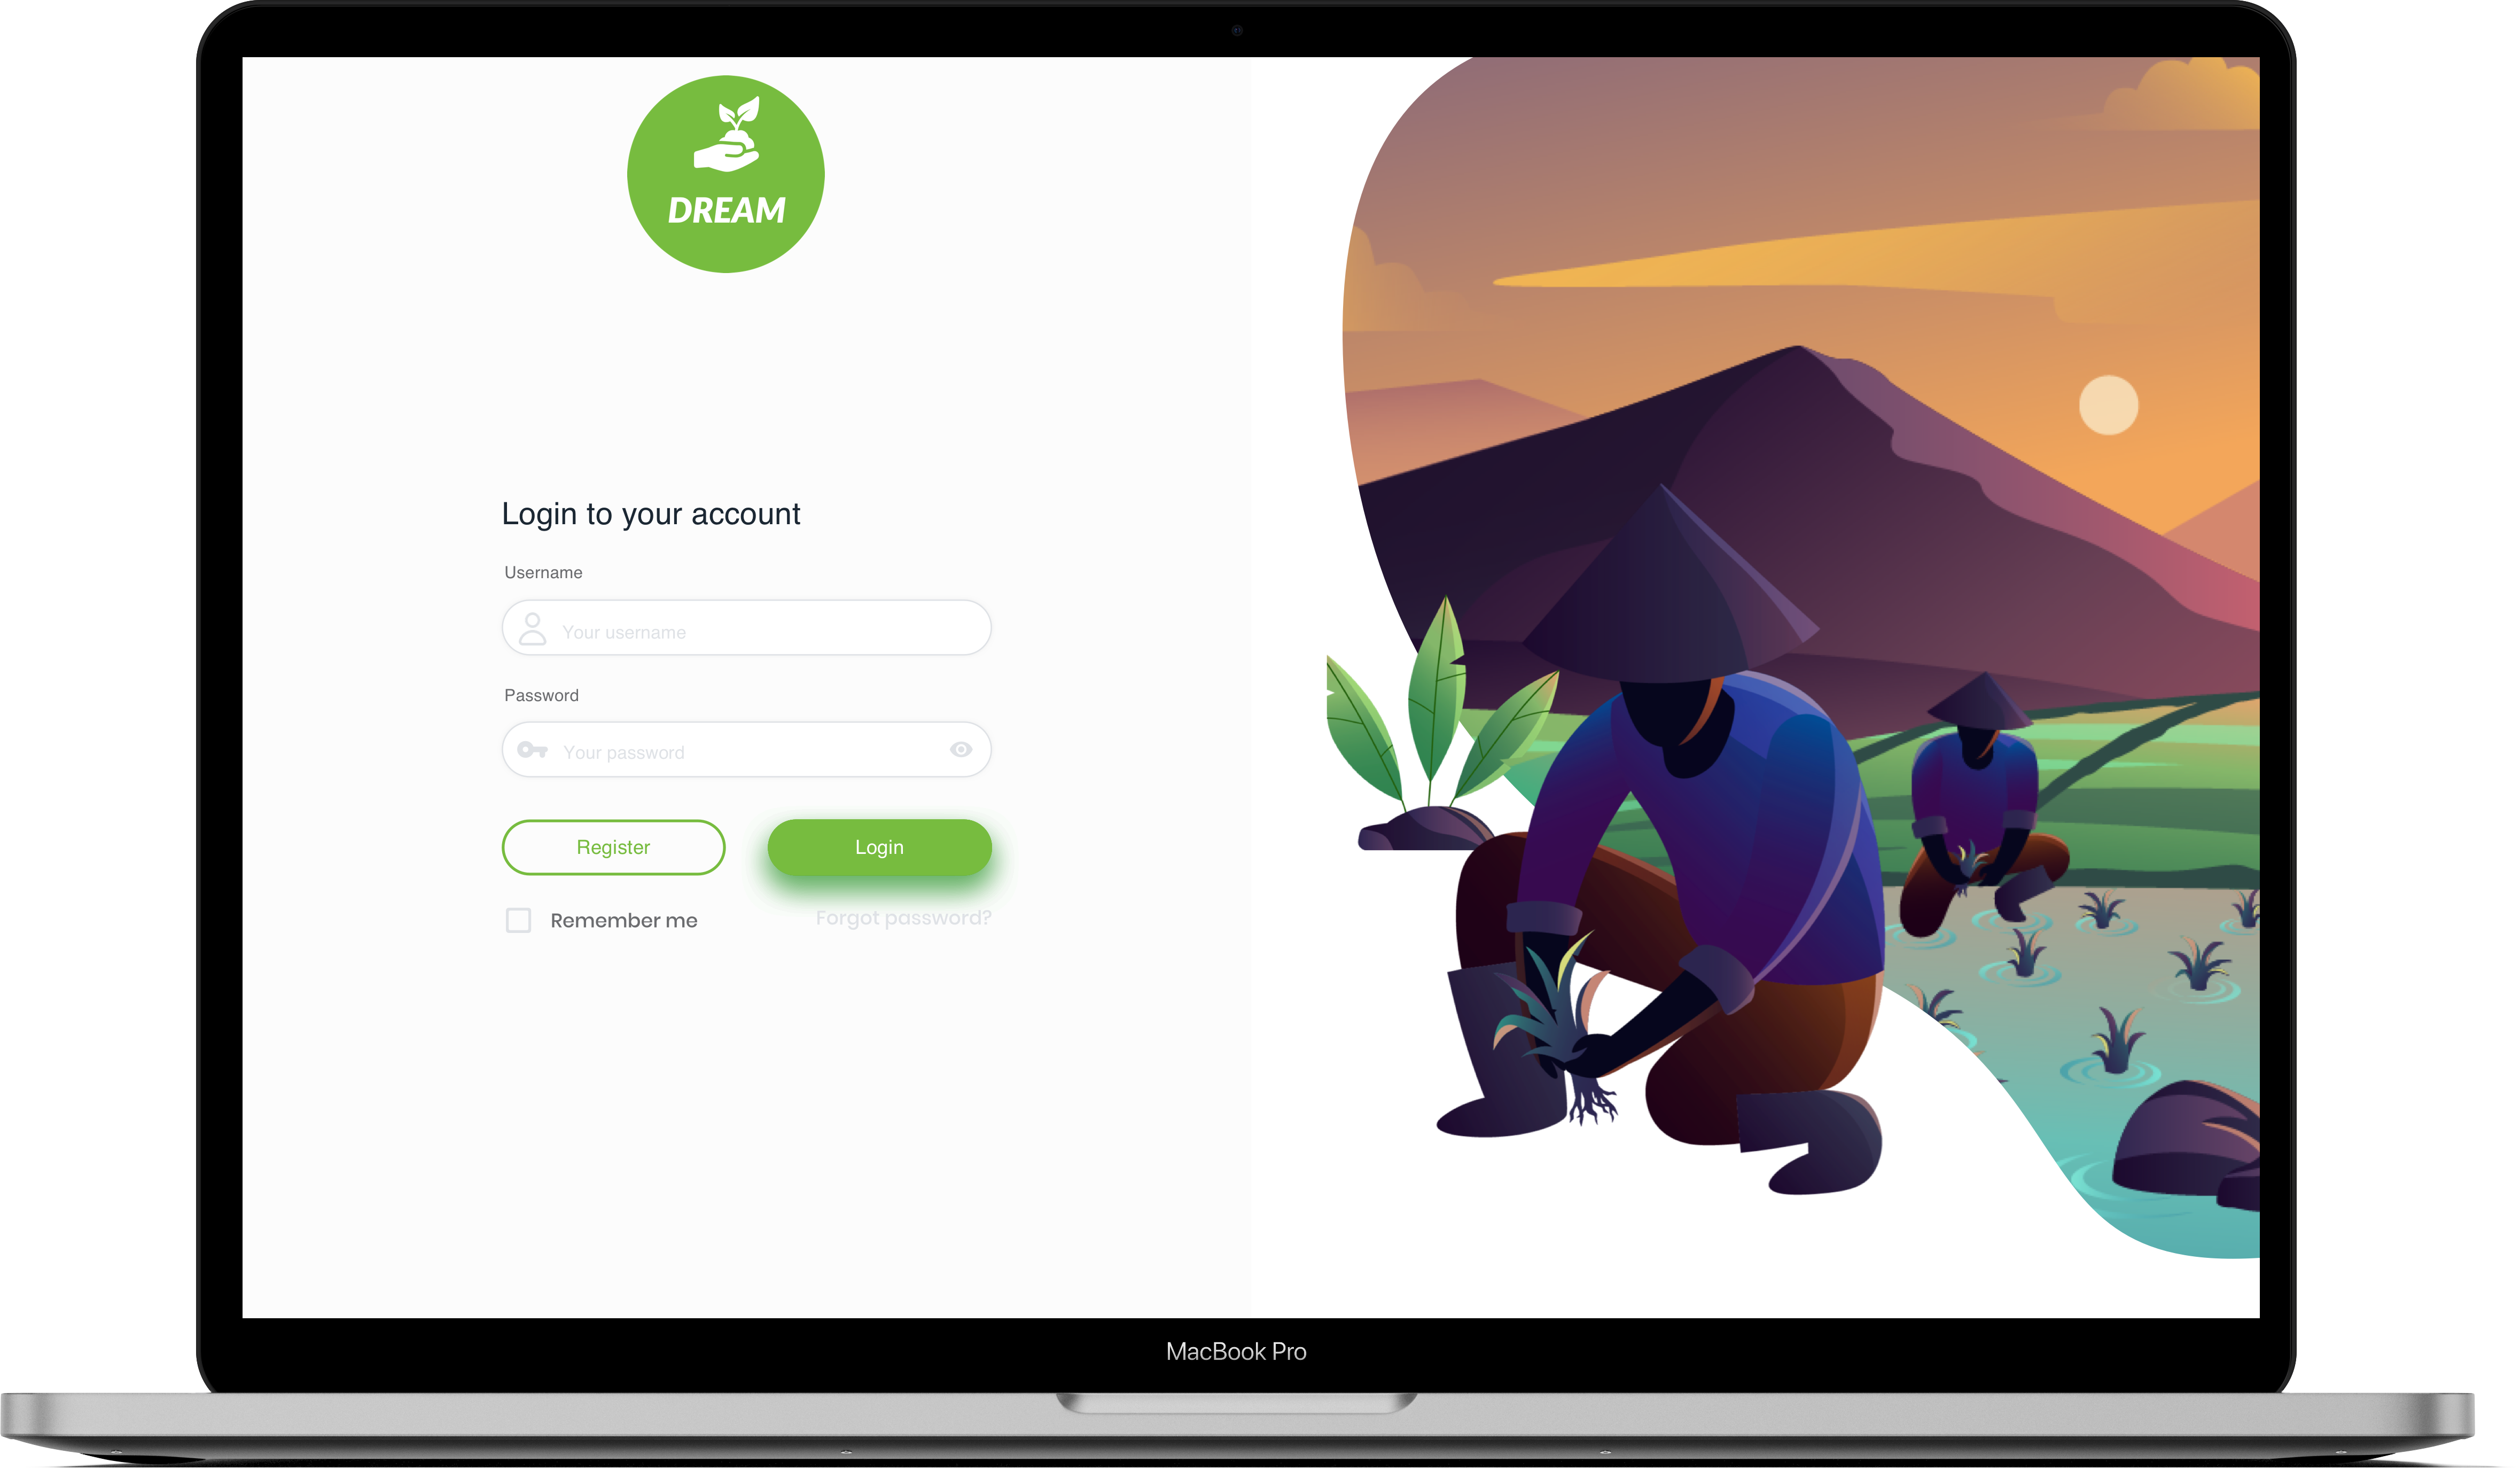
\includegraphics[width=140mm,scale=0.9]{./Images//Mocks/WebApp/Login.png}
  \caption{WebApp Login page}
\end{figure}

The three actors of DREAM can access to the application through this login page. If they do not yet have an account, they can simply access the registration page via an appropriate button.

\subsubsection{WebApp Policy Maker Homepage}

\begin{figure}[H]
  \centering
  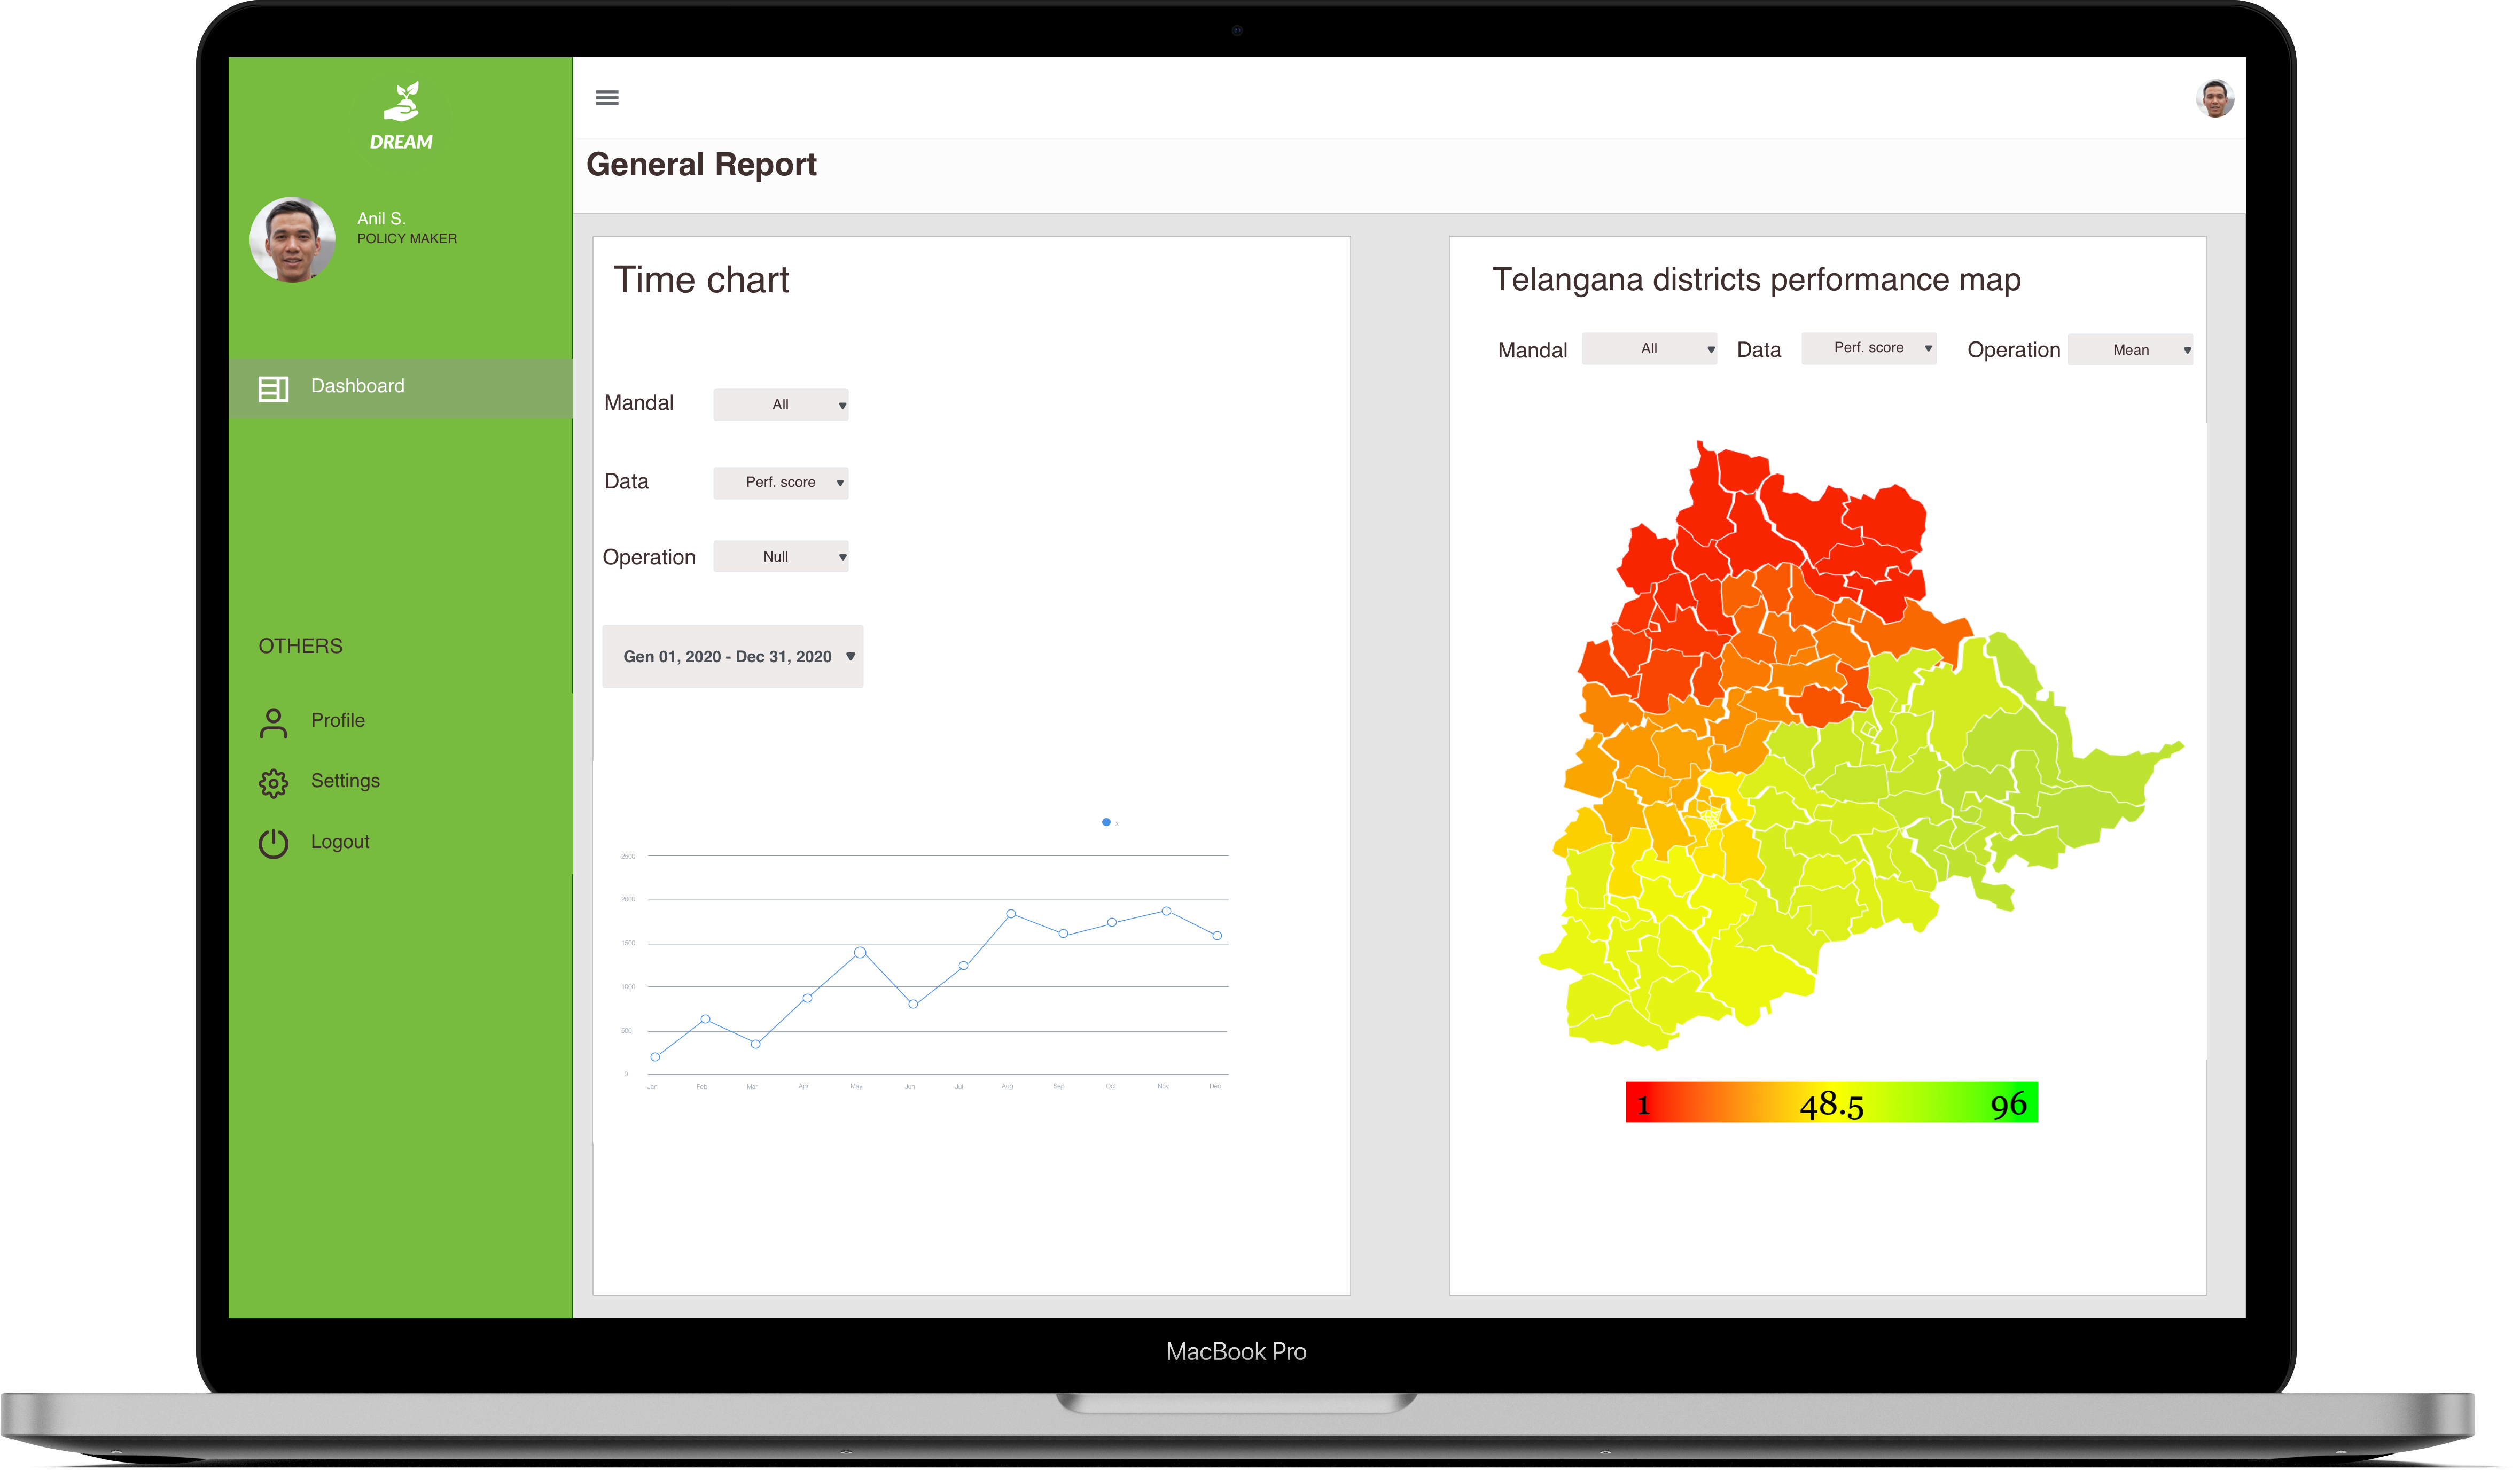
\includegraphics[width=140mm,scale=0.9]{./Images//Mocks/WebApp/PolicyMaker.png}
  \caption{WebApp Policy Maker Homepage}
\end{figure}

This is PolicyMaker homepage (in \textit{Figure 3.3} called "Dashboard") where the he/she can generate a time chart according to some inputs, and can also visualize Telangana's farmers performance map using some filters.

\subsubsection{WebApp Agronomist Homepage}

\begin{figure}[H]
  \centering
  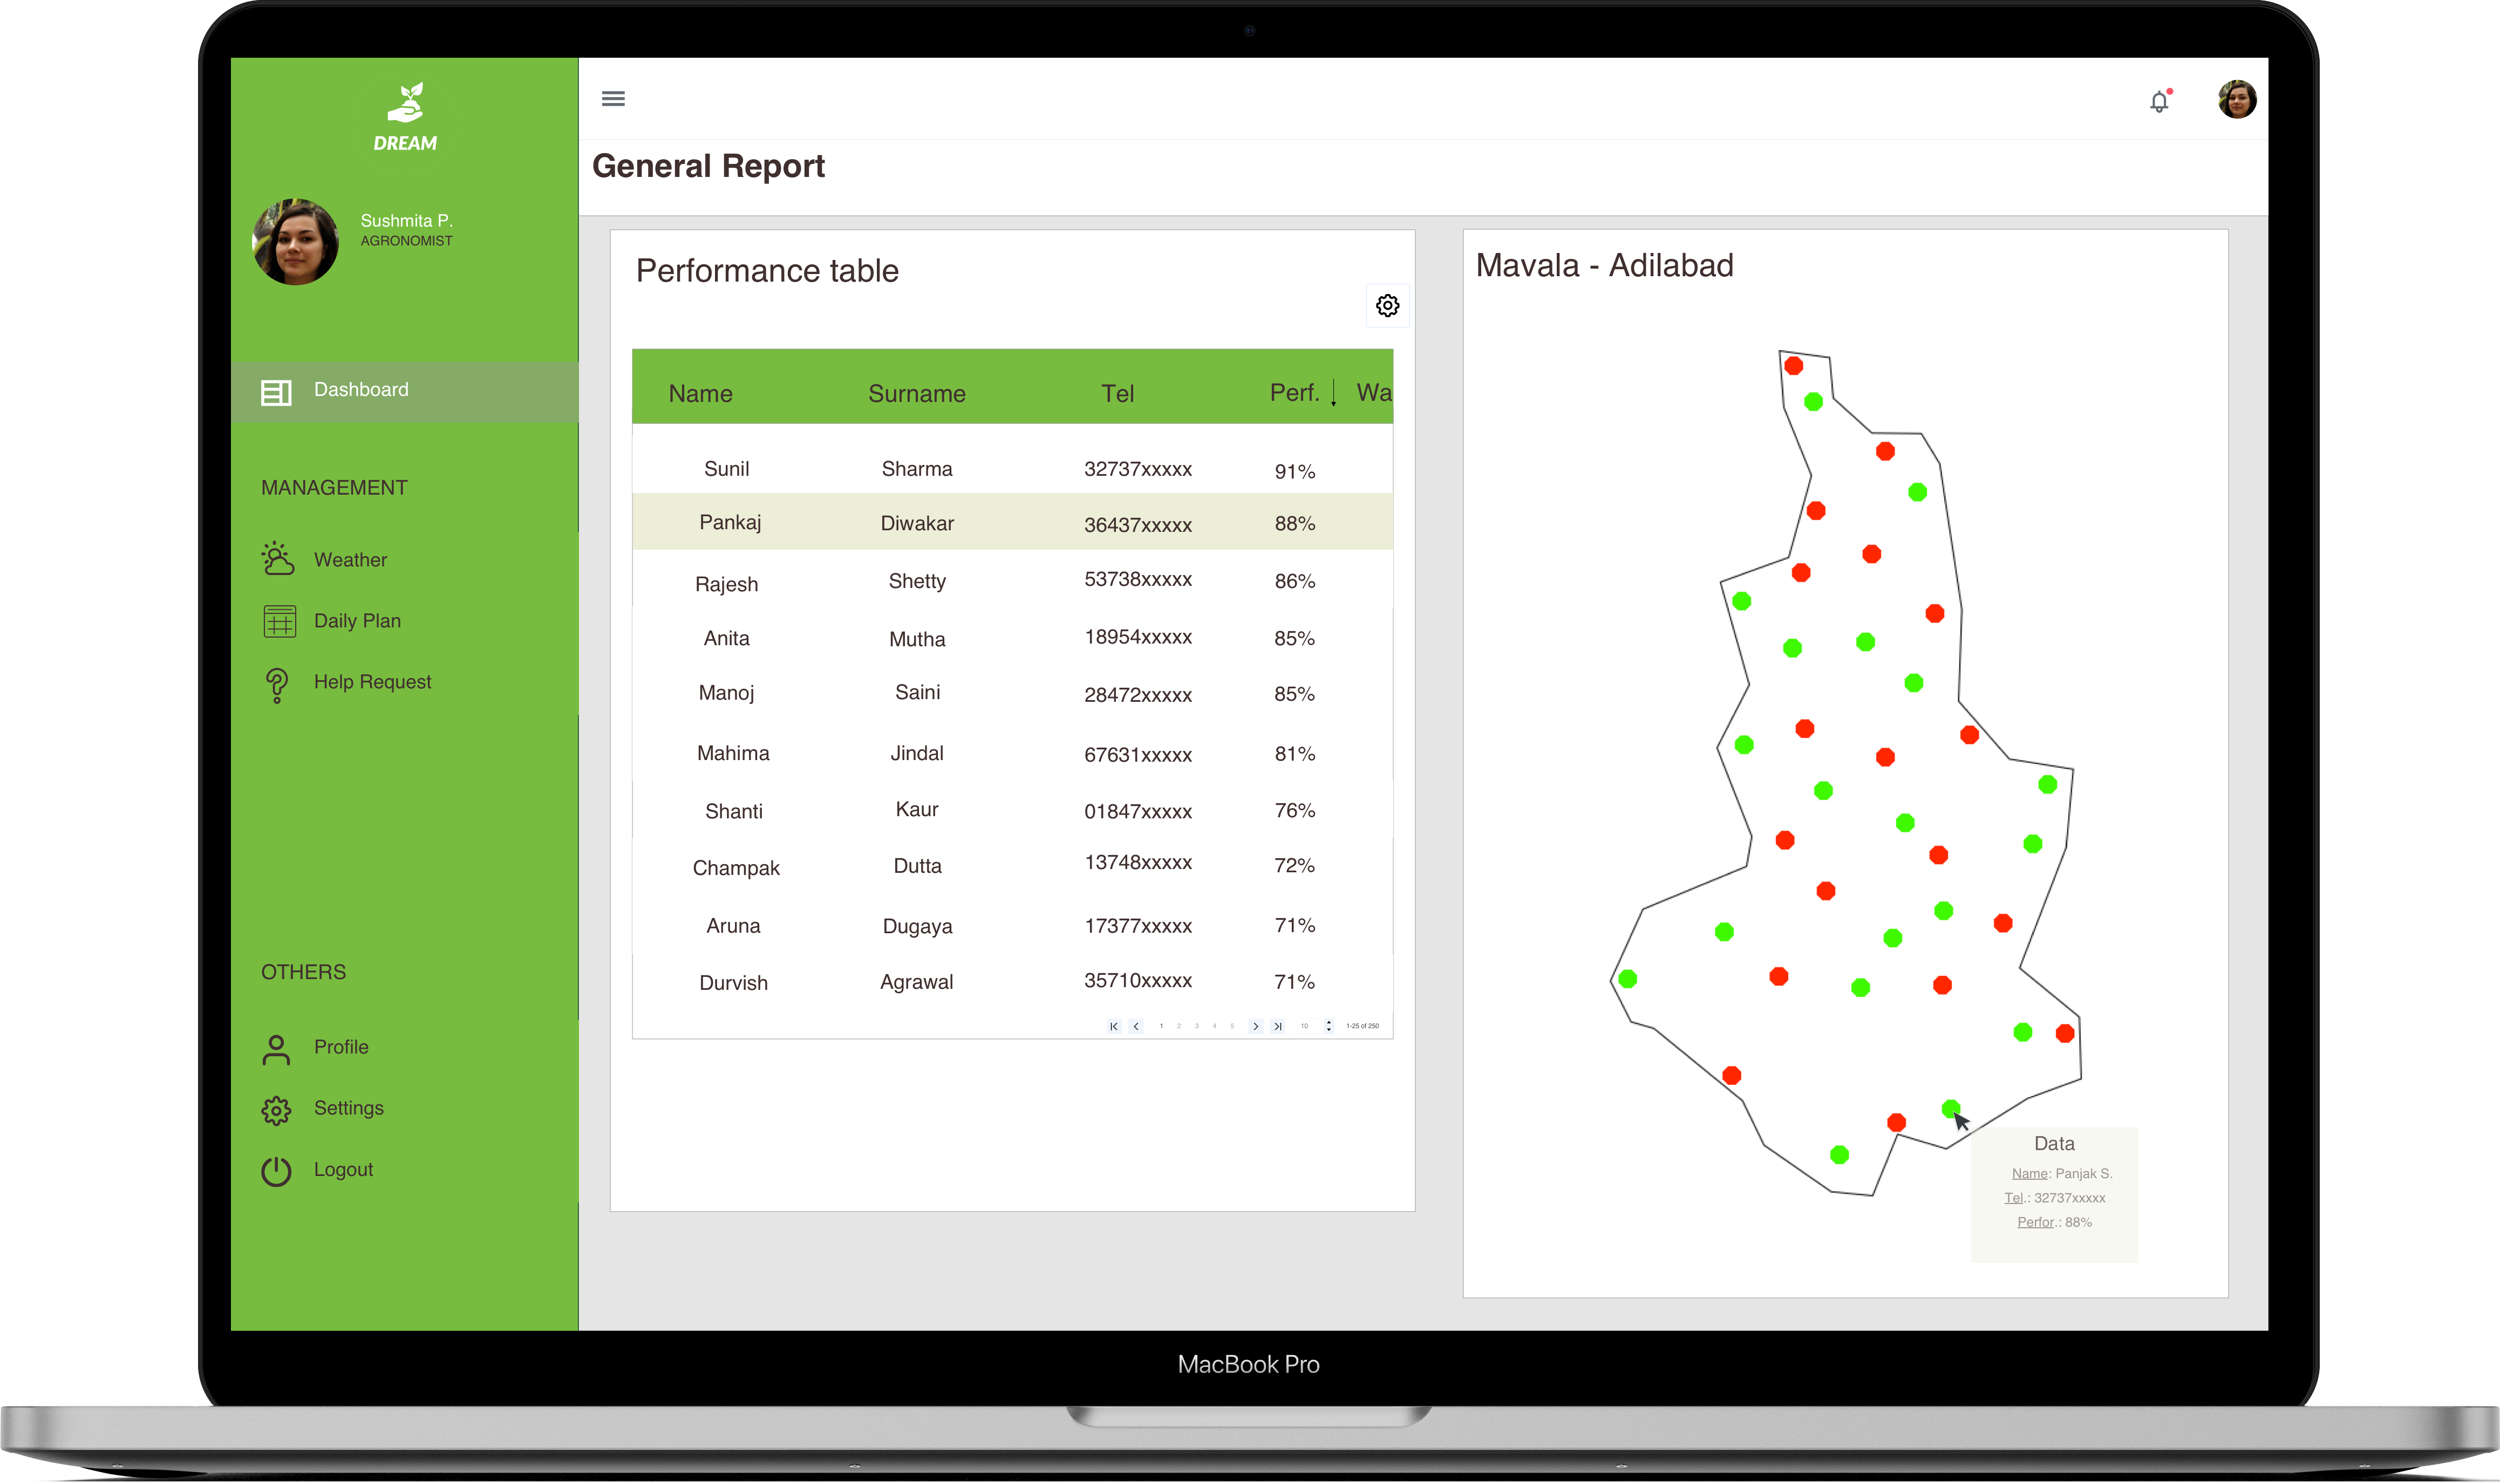
\includegraphics[width=140mm,scale=0.9]{./Images//Mocks/WebApp/Agronomist_Home.png}
  \caption{WebApp Agronomist Homepage}
\end{figure}

This is Agronomist homepage (in \textit{Figure 3.4} called "Dashboard") where he/she can view his/her mandal's farmer performance on a map, and he/she can also view some info about a farmer by pointing mouse cursor on a point, and the performance table, that resume, in descending order (by performance score), info's about farmers.

\subsubsection{WebApp Agronomist Weather Conditions page}

\begin{figure}[H]
  \centering
  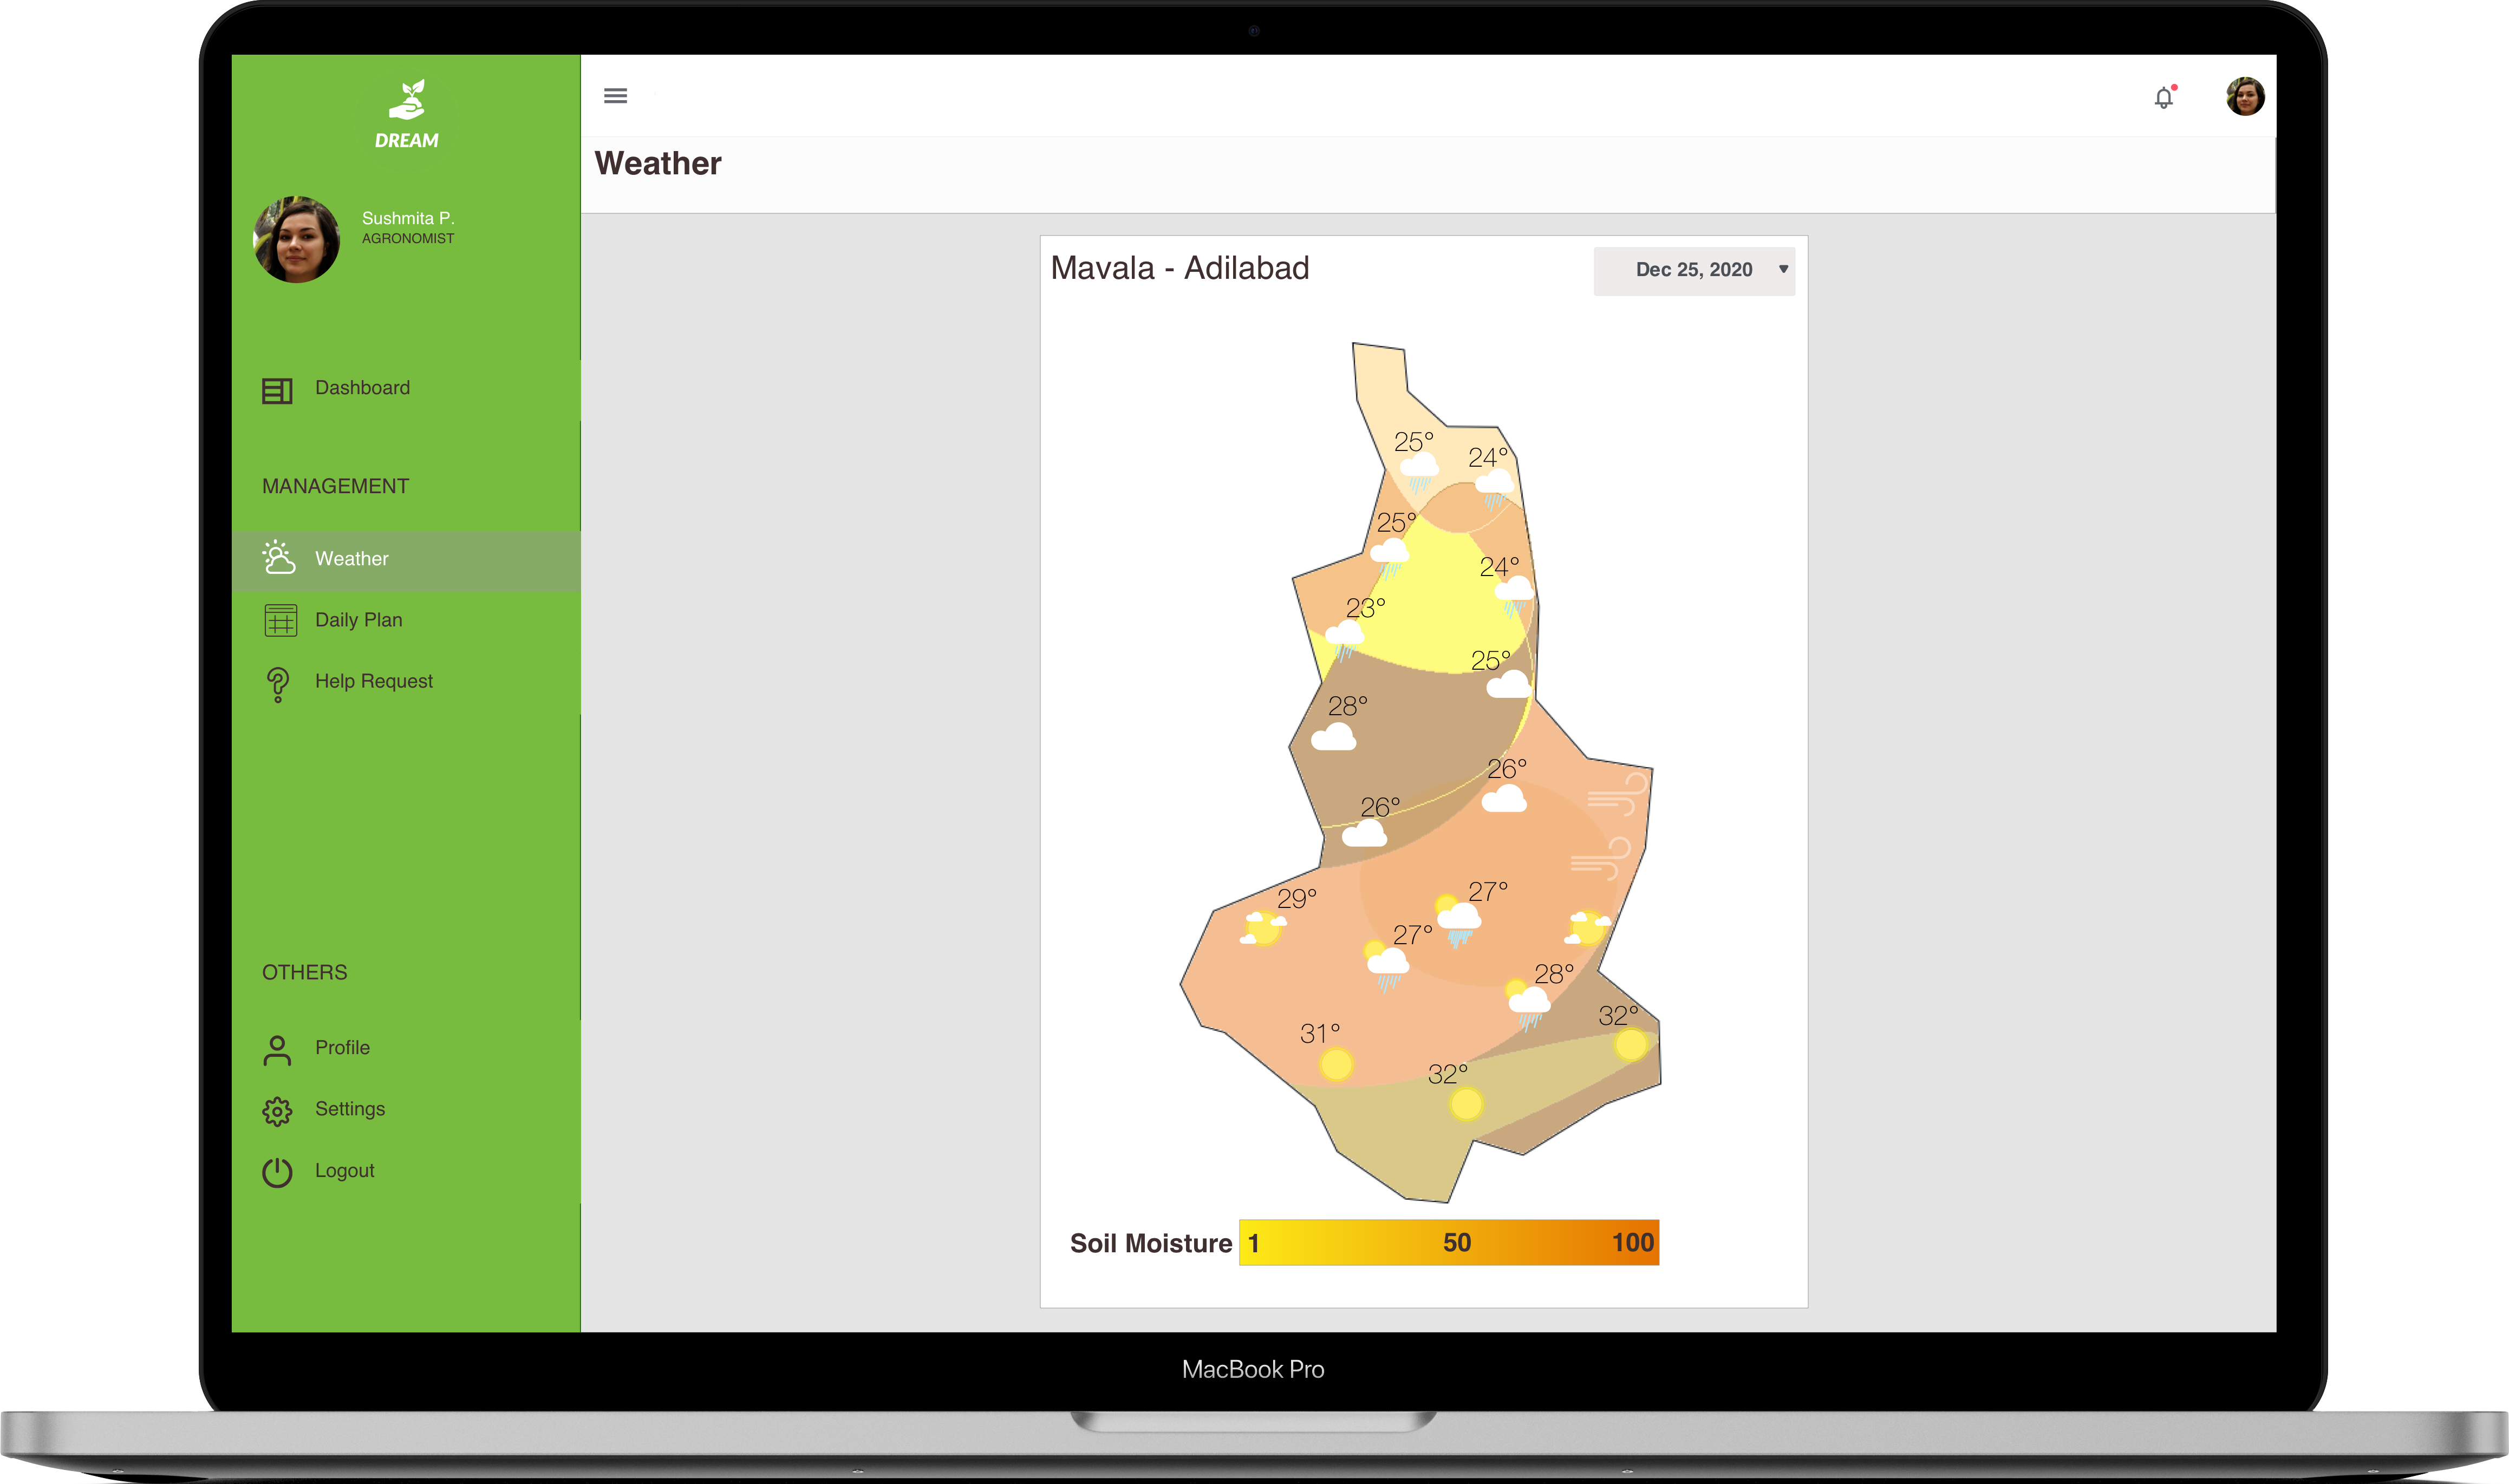
\includegraphics[width=140mm,scale=0.9]{./Images//Mocks/WebApp/Agronomist_Weather.png}
  \caption{WebApp Agronomist Weather Conditions page}
\end{figure}

This is Agronomist weather page, where he/she can visualize info about weather conditions and soil moisture of his/her mandal. He/she can also view information about weather forecasts in the next seven days by setting it into the menu.

\subsubsection{WebApp Farmer Homepage}

\begin{figure}[H]
  \centering
  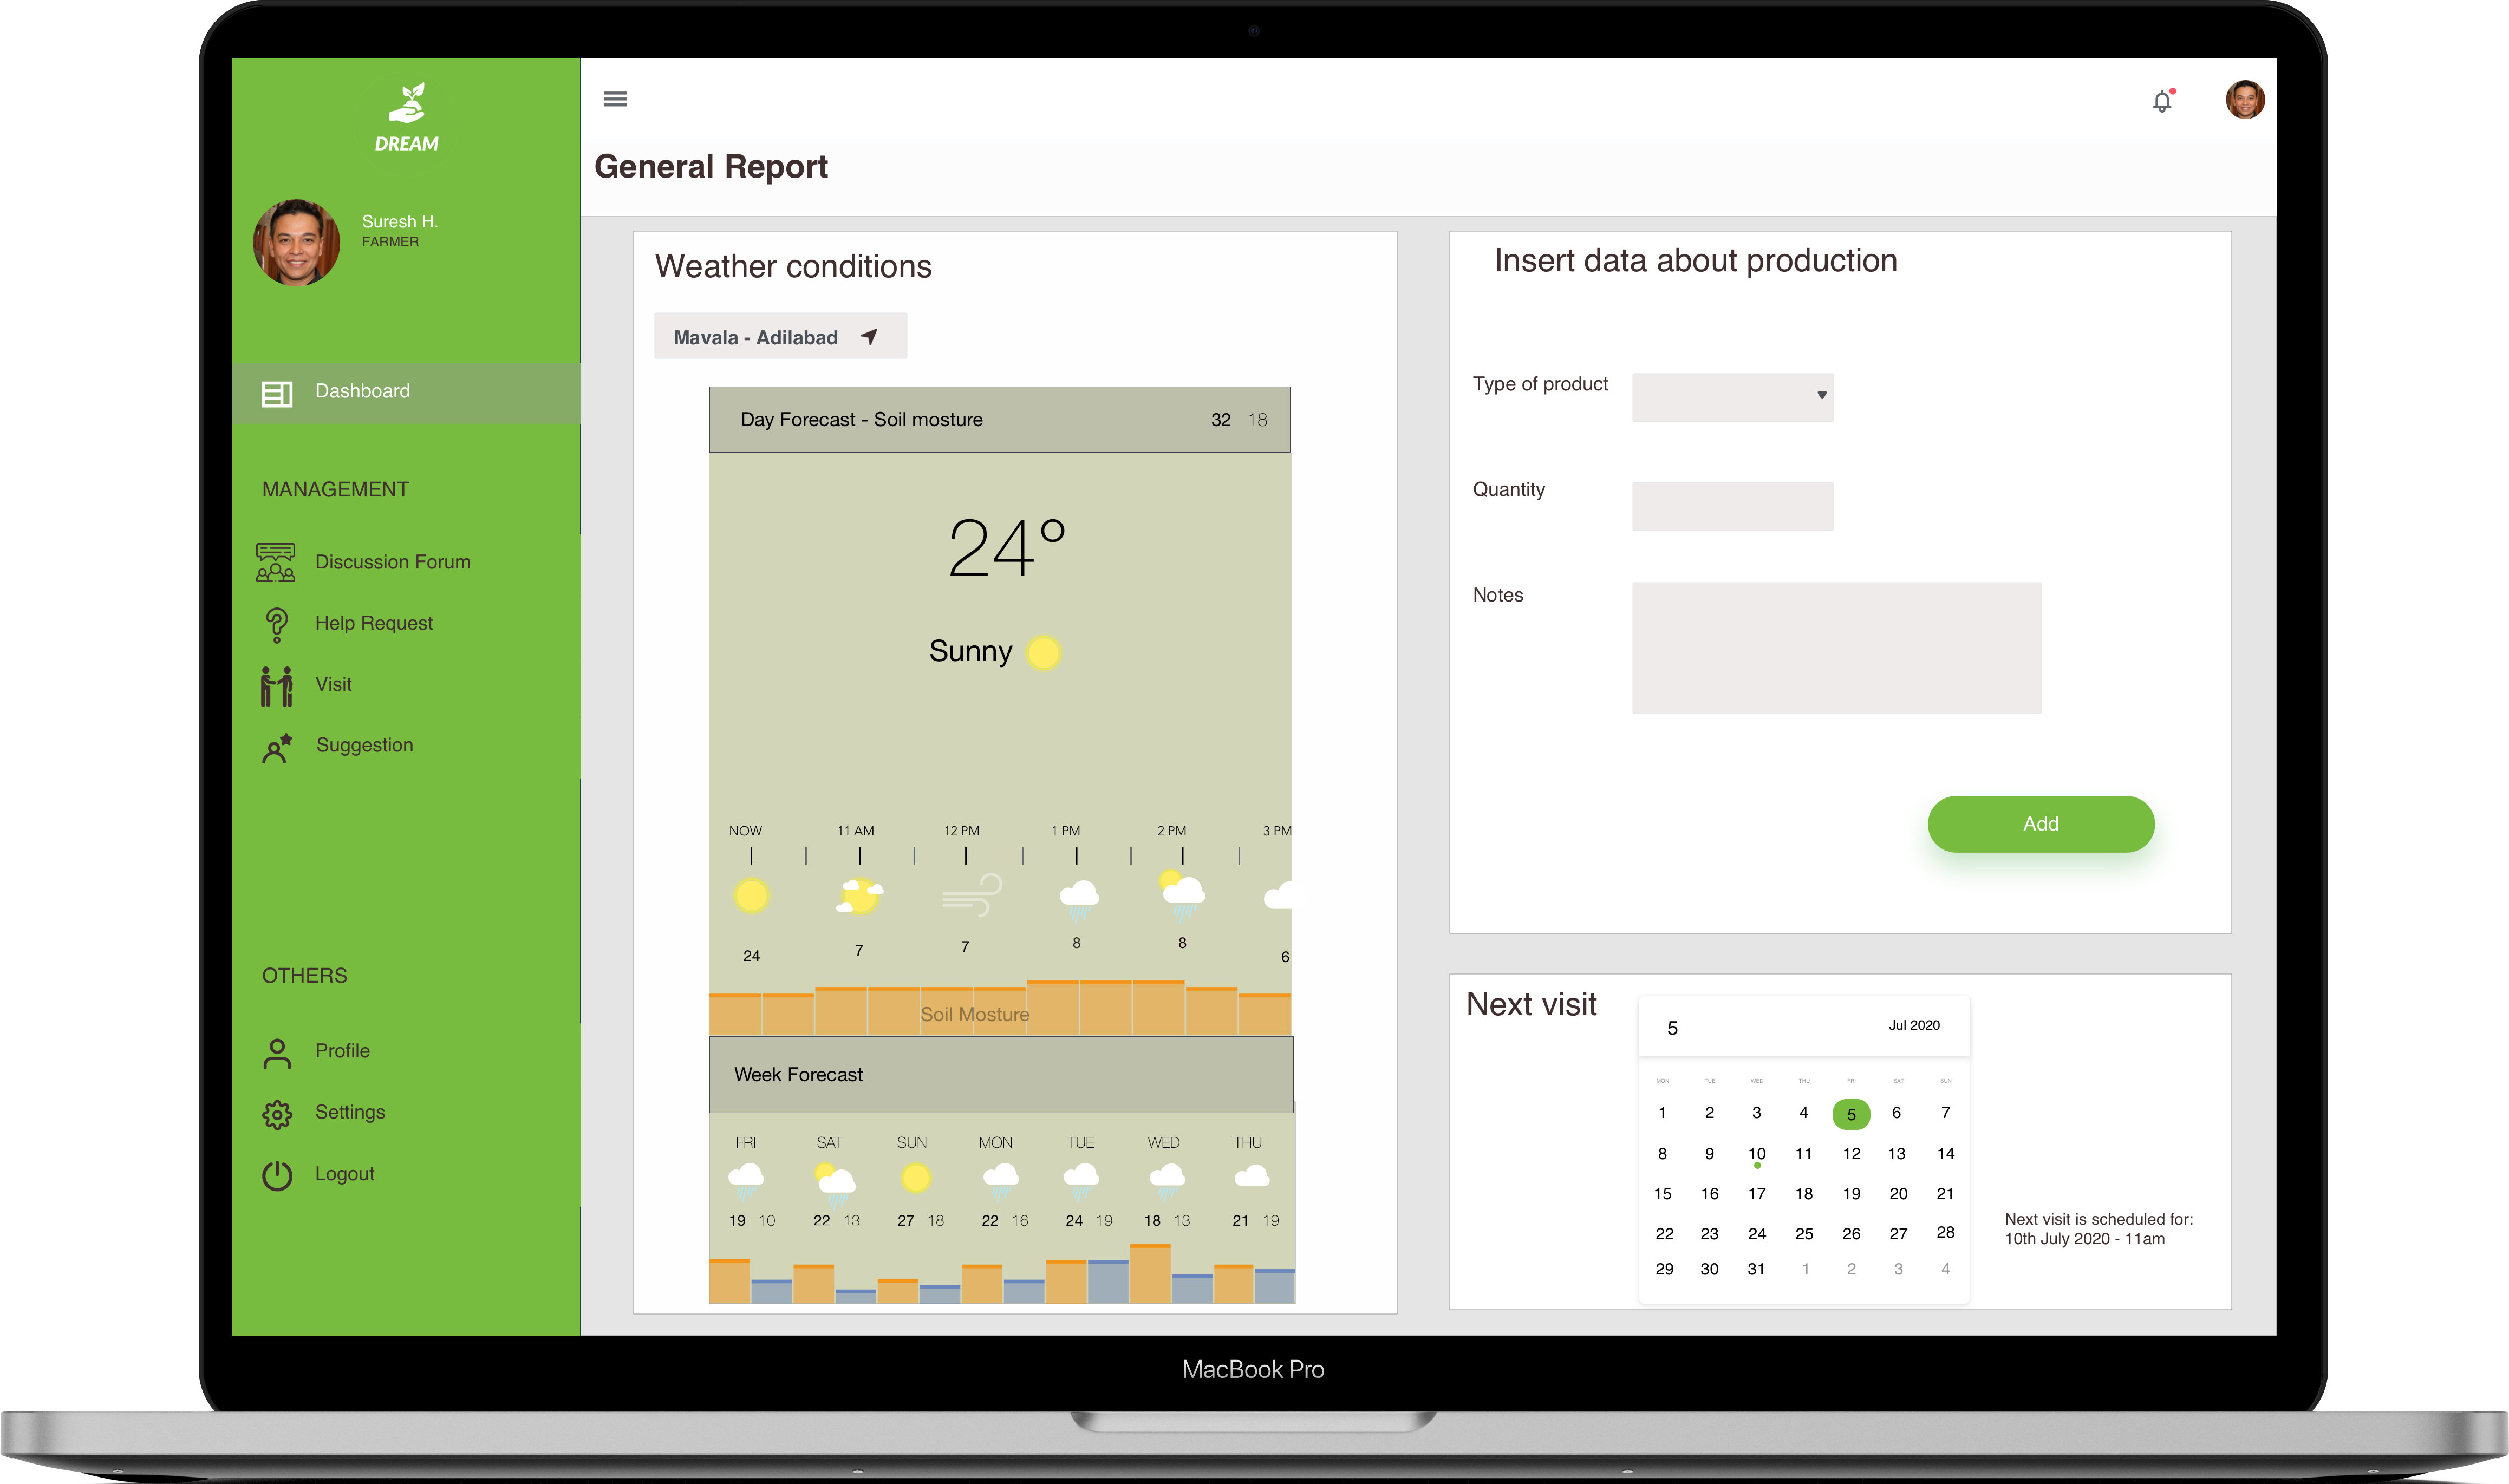
\includegraphics[width=140mm,scale=0.9]{./Images//Mocks/WebApp/Farmer_Home.png}
  \caption{WebApp Farmer Homepage}
\end{figure}

This is Farmer homepage (in \textit{Figure 3.6} called "Dashboard") where he/she can visualize weather forecast and soil moisture based on her/his location, he/she can insert data about his/her production and can visualize on the calendar the next visit scheduled by his/her mandal's responsible agronomist.

\subsubsection{WebApp Farmer Discussion Forum page}

\begin{figure}[H]
  \centering
  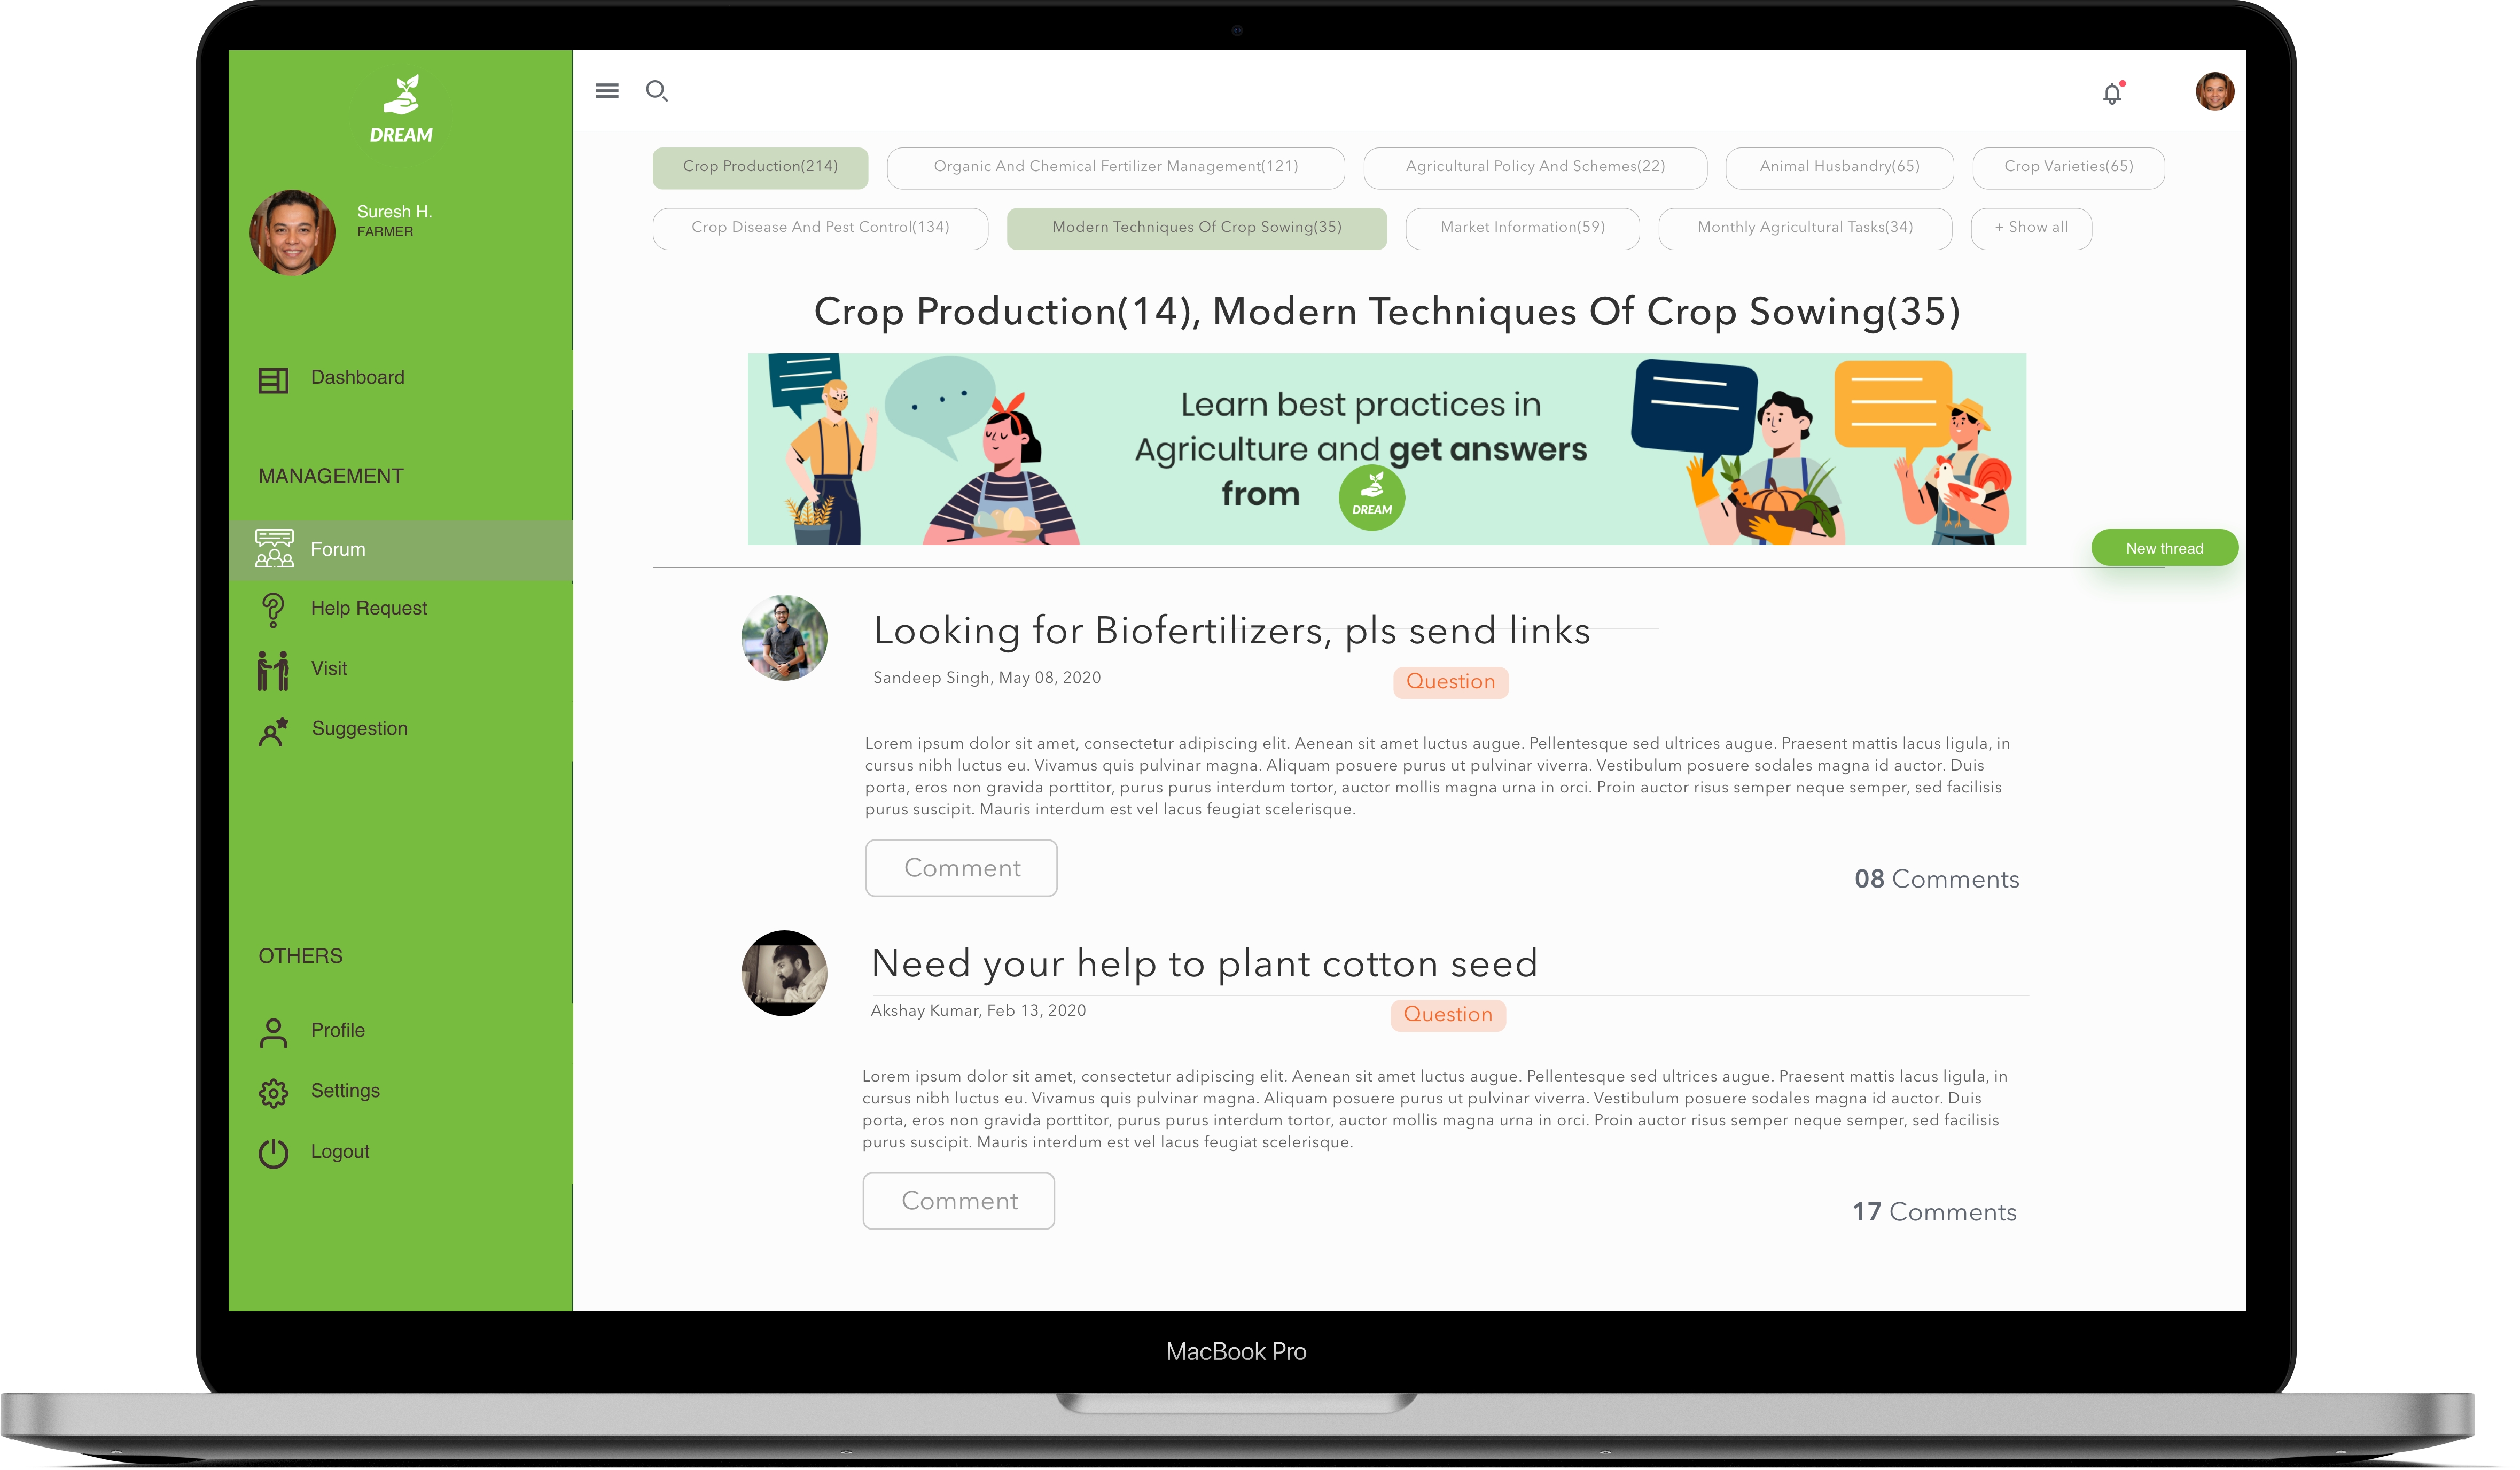
\includegraphics[width=140mm,scale=0.9]{./Images//Mocks/WebApp/Farmer_Forum.png}
  \caption{WebApp Farmer Discussion Forum page}
\end{figure}

This is Farmer forum section, where he/she can interact with other farmers by opening new threads or replying to existing one.
He/she can also look up for a thread using search function.

\subsubsection{MobileApp Login and Registration page}

\begin{figure}[H]
  \begin{minipage}{0.5\textwidth}
  \centering
    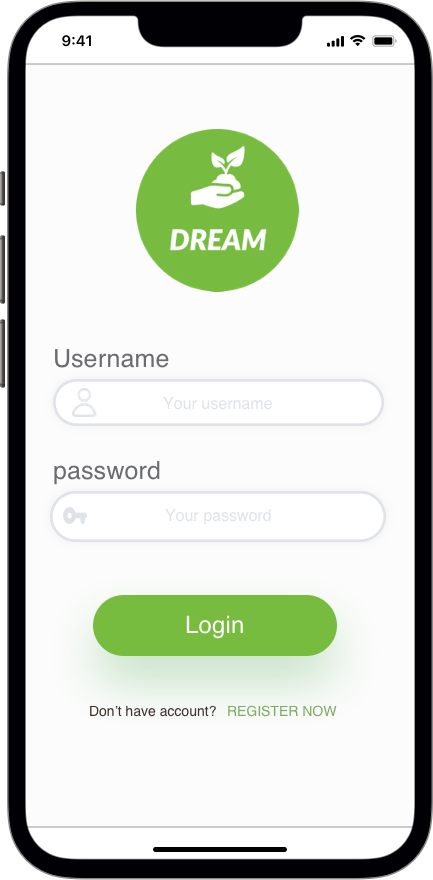
\includegraphics[width=40mm,scale=0.9]{./Images//Mocks/Mobile/Login.png}
    \caption{Mobile Login page}
    \end{minipage}
\hfill
   \begin{minipage}{0.5\textwidth}
     \centering
     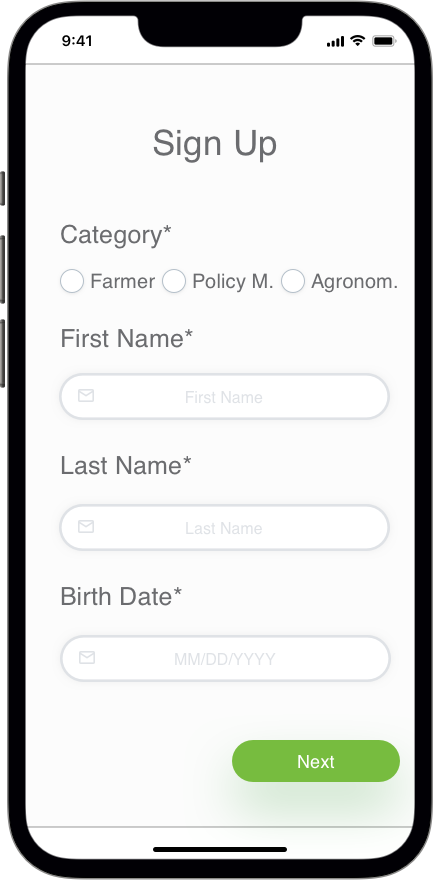
\includegraphics[width=40mm,scale=0.9]{./Images//Mocks/Mobile/Registration.png}
     \caption{Mobile Registration page}
   \end{minipage}
\end{figure}

\subsubsection{MobileApp Farmer Menu}

\begin{figure}[H]
  \centering
     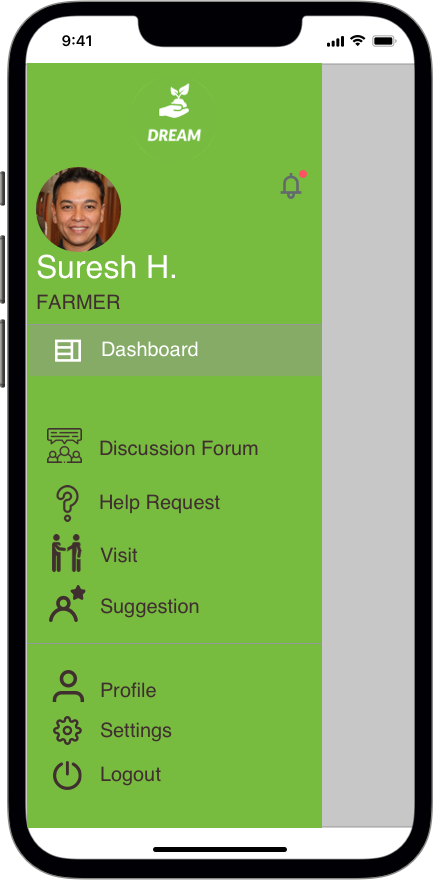
\includegraphics[width=40mm,scale=0.9]{./Images//Mocks/Mobile/Farmer_menu.png}
     \caption{MobileApp Farmer Menu}
\end{figure}

Interface that shows the menu of actions that a farmer can perform in the application.\\

\subsubsection{MobileApp Farmer Help Request page}

\begin{figure}[H]
  \centering
   \begin{minipage}{0.4\textwidth}
     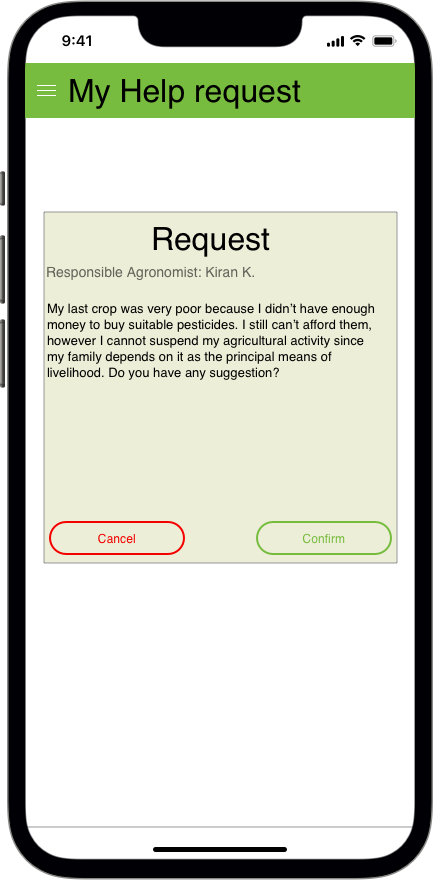
\includegraphics[width=40mm,scale=0.9]{./Images//Mocks/Mobile/Farmer_help_req.png}
     \caption{MobileApp Farmer Help Request page}
   \end{minipage}
    \hfill
   \begin{minipage}{0.4\textwidth}
     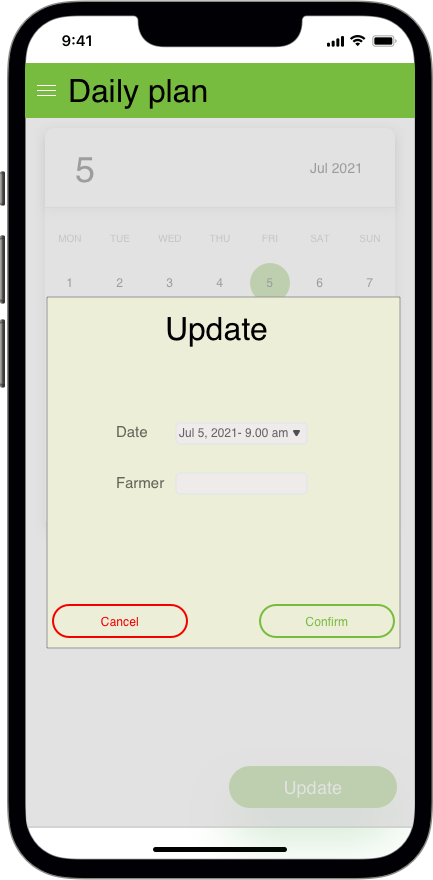
\includegraphics[width=40mm,scale=0.9]{./Images//Mocks/Mobile/Agronomist_daily_plan.png}
     \caption{Mobile Agronomist daily plan}
   \end{minipage}
\end{figure}

\begin{itemize}
    \item \textbf{Figure 3.12: Mobile Farmer help request}\\ 
    \textcolor{red}{Interface that shows an example of help request made by a Farmer with only the associated Agronomist as recipient.}
\end{itemize}
\begin{itemize}
    \item \textbf{Figure 3.13: Mobile Agronomist daily plan}\\ 
    \textcolor{red}{Interface that shows an example of update of the daily plan made by an Agronomist.}
\end{itemize}
\newpage

\begin{figure}[H]
  \centering
     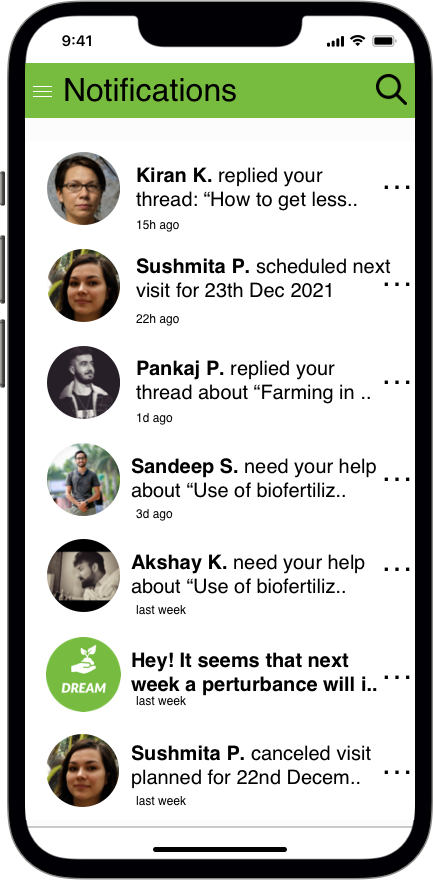
\includegraphics[width=40mm,scale=0.9]{./Images//Mocks/Mobile/Farmer_notif.png}
     \caption{Mobile Farmer notifications}
\end{figure}

\newpage


\begin{itemize}
    \item \textbf{Figure 3.11: Mobile Farmer notifications}\\ 
    \textcolor{red}{Interface that shows various kind of notifications received by a Farmer: suggestions, visits scheduled by an Agronomist, reply to a help request, reply on the discussion forum.}
\end{itemize}
\newpage